\documentclass[10pt,a4paper]{article}

\usepackage[utf8x]{inputenc}
\usepackage[norsk]{babel}
\usepackage[T1]{fontenc,url}
\usepackage[hang,small,bf]{caption}
\usepackage{relsize}
\usepackage{setspace}
\usepackage{parskip}
\usepackage{lmodern}
\usepackage{microtype}
\usepackage{verbatim}
\usepackage{amsmath, amssymb, amsthm}
\usepackage{mathtools}
\usepackage{tikz}
\usepackage{physics}
\usepackage{algorithm}
\usepackage{algpseudocode}
\usepackage{listings}
\usepackage{enumerate}
\usepackage{graphicx}
\usepackage{float}
\usepackage{hyperref}
\usepackage{varioref}
\usepackage{todonotes}
\usepackage{color}
\usepackage{siunitx}
\usepackage[margin=1.5cm]{geometry}
\labelformat{equation}{ligning~(#1)}

\renewcommand{\exp}{\mathrm{e}^}
\newcommand{\halflife}{t_{\frac{1}{2}}}

\definecolor{light_green}{rgb}{0, 0.6, 0}
\definecolor{light_grey}{rgb}{0.5, 0.5, 0.5}
\definecolor{magenta}{rgb}{0.7, 0, 0.5}


\lstdefinestyle{py}{
    language = python,
    frame = single,
    showstringspaces = false,
    basicstyle = \small\ttfamily,
    breaklines = true,
    commentstyle = \color{light_grey},
    keywordstyle = \color{magenta},
    stringstyle = \color{light_green},
}


\begin{document}
\section*{Oppgave 8.1}
Her er poenget at de skal kunne generere tilfeldige verdier som er like sannsynlige å få, og bruke disse. Det er helt greit om de ikke bruker vektoriserng for å teste, men det hadde vært fint om de ble fortalt at dette finnes. 
\lstinputlisting[style=py]{check_energy_conservation.py}


\newpage
\section*{Oppgave 8.2}
Det viktige her er at de på en eller annen måte har en array av 0'er og 1'ere, som de looper over og flipper med en random test. Det totale antallet 1'ere ved hvert tidssteg skal så lagres i en ny array. Det er ikke lov å på en eller annen måte basere seg på den analytiske formelen.

Et typisk plott for $N = 40$ atomer er vist under, men merk at dette kan se ganske annerledes ut pga tilfeldigheter. Plottet skal konvergere godt mot den analytiske løsningen for store N (type $N>1000$).
\lstinputlisting[style=py]{random_decay.py}

\begin{figure}[H]
\centering
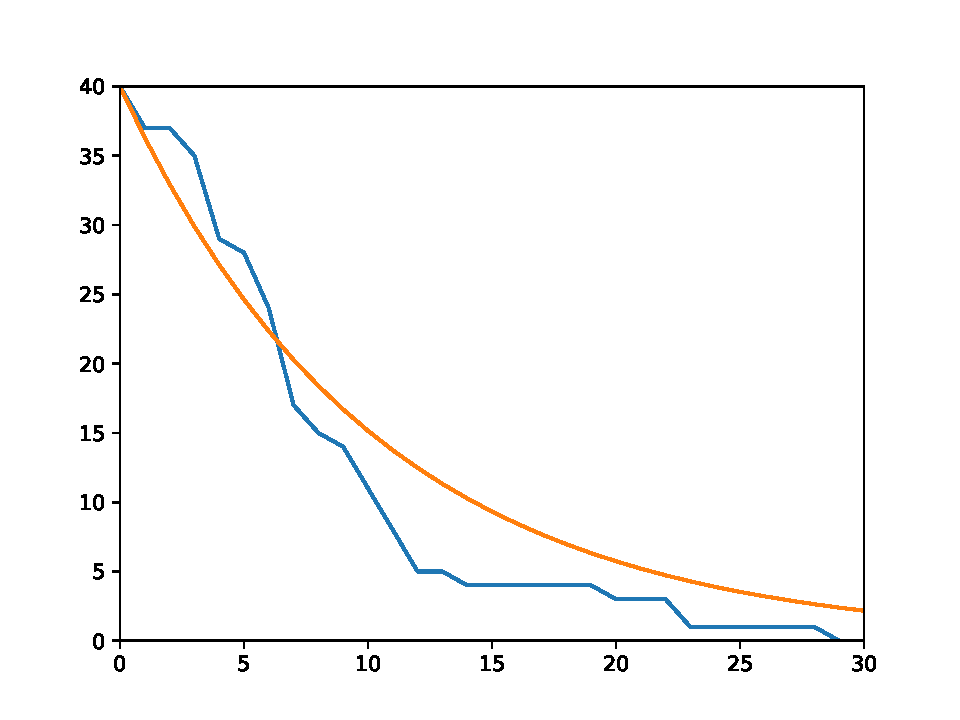
\includegraphics[width=0.8\textwidth]{fig_random_decay.pdf}
\end{figure}

\newpage
\section*{Oppgave 8.3}
Siden vi generer ganske mange verdier, er sannsynligheten veldig liten for at listen med treffvinkler blir tom. Har de sett bort i fra å sjekke om listen er tom, men fått til alt annet i oppgaven, er det helt greit å se bort i fra dette.

Det er heller ikke fullt så viktig om de husker å ta med en kommentar på om de ser forskjell i antall treffvinkler for a) og b). 
\lstinputlisting[style=py]{optimal_angles_shoot.py}
\begin{verbatim}
>>> Number of found alphas using uniform: 20
>>> Number of found alphas using normal with mean = 0.755561: 329
\end{verbatim}

\newpage
\section*{Oppgave 8.4}
Hele fremgangsmåten er ganske nøyaktig beskrevet i oppgaven. Resultatet av å plukke et random element i listen vår skal være en liste på 3 elementer.

I oppgave b) er det ikke krav om å implementere en testfunksjon. Det skal bare summes over listen, og sammenlignes med analytisk verdi.
\lstinputlisting[style=py]{gaussian_velocities.py}

\begin{verbatim}
>>> [ -0.35447337  -4.79488557 -11.6815135 ]
>>> 1.21330434569e-19 1.242e-19
\end{verbatim}


\pagebreak
\section*{Oppgave 8.5}
Her skal de bli kjent med fordelene ved å bruke vektorisering. Det nye er tidstakingen.

 Ellers, er det ikke noe annet som er spesielt ved denne oppgaven. Hvis de har fått til enten a eller b, men ikke begge, så mister oppgaven litt hensikt - meningen er tross alt å bli kjent med forskjellene mellom vektoriserte funksjoner og 'standarde' funksjoner. 
\lstinputlisting[style=py]{raindrops.py}
Resultat etter en kjøring (kun veiledene - verdiene kan jo variere):
\begin{verbatim}
>>> Average vT = 11.9873 m/s
    Time used w/o numpy: 0.237353 seconds
>>> Average vT = 11.9739 m/s
    Time used with numpy: 0.00913 seconds
\end{verbatim}





















\end{document}


